\documentclass{beamer}
\mode<presentation> {\usetheme{default}}
%\setbeamersize{text margin left=10mm,text margin right=10mm}


\setbeamertemplate{footline}[frame number]

\usepackage{amssymb}
\usepackage{amsthm}
\usepackage{amsmath}
\usepackage{booktabs}
\usepackage{needspace}
\usepackage{comment}
\usepackage{tikz}
\usepackage{graphicx}
\usepackage{bbm, dsfont}

\usetikzlibrary{arrows,shapes,calc,positioning}

\theoremstyle{plain}
\newtheorem{thm}{Theorem}[section]
\newtheorem{cor}[thm]{Corollary}
\newtheorem{lem}[thm]{Lemma}
\newtheorem{prop}[thm]{Proposition}
%
\theoremstyle{definition}
\newtheorem{defn}{Definition}[section]
\newtheorem{remk}{Definition}[section]
\newtheorem{exam}{Example}[section]
\newtheorem{prob}{Exercise}[section]
\newtheorem{solu2}{Solution}[section]
\newenvironment{Shaded}{\begin{snugshade}}{\end{snugshade}}

\newcommand{\dif}{\operatorname{d}}
\newcommand{\var}{\operatorname{Var}}
\newcommand{\blue}[1]{\textcolor{blue}{#1}}
\newcommand{\purple}[1]{\textcolor{purple}{#1}}

% Sections of Chapter 5 are numbered 5.1, 5.2, ..., 5.5
\renewcommand{\thesection}{5.\arabic{section}}

% Actuarial angle: a_{\ang{n}i} gives a-angle-n at i
\newcommand{\ang}[1]{\overline{#1|}}

% Simple timeline: \timeline{length}{list of position/label pairs}
\newcommand{\timeline}[2]{%
  \begin{tikzpicture}
    \draw (0,0) -- (#1,0);
    \foreach \x/\lab in {#2} {
      \draw (\x,0.12) -- (\x,-0.12);
      \node[below] at (\x,-0.12) {\footnotesize $\lab$};
    }
  \end{tikzpicture}%
}

% Cash-flow timeline: \cftimeline{length}{position/time-label pairs}{position/payment-label pairs}
\newcommand{\cftimeline}[3]{%
  \begin{tikzpicture}
    \draw (0,0) -- (#1,0);
    \foreach \x/\lab in {#2} {
      \draw (\x,0.12) -- (\x,-0.12);
      \node[below] at (\x,-0.12) {\footnotesize $\lab$};
    }
    \foreach \x/\lab in {#3} {
      \node[above] at (\x,0.12) {\footnotesize $\lab$};
    }
  \end{tikzpicture}%
}
\newcommand{\green}[1]{\textcolor{green!50!black}{#1}}
\newcommand{\red}[1]{\textcolor{red}{#1}}
%opening

\title{RISK 201: Repayment of Debts}
\author{Himchan Jeong, FSA}
\institute{Department of Statistics \& Actuarial Science \\Simon Fraser University}
\date{}

\begin{document}
\maketitle

%======================================================================
\section{Amortization of a debt}
%======================================================================

\begin{frame}{5.1 Amortization of a debt}

\begin{itemize}
\item When the \textbf{amortization method} is used to repay a loan, the borrower makes \textbf{installment payments} to the lender at regular intervals.
\medskip
\item Each installment payment is used:
  \begin{itemize}
  \item to pay the interest on the outstanding loan balance since the last payment, AND
  \item to repay part of the principal borrowed.
  \end{itemize}
\medskip
\item We will be interested in finding the outstanding balance, and the interest/principal portion of each payment.
\end{itemize}

\end{frame}

\begin{frame}{Amortization schedule}

\begin{itemize}
\item An \textbf{amortization schedule} for a loan identifies the corresponding portions of each payment.
\medskip
\item Dividing each payment into principal and interest is often required in practice. For example, the two may be treated differently for income tax purposes.
\medskip
\item Amortization schedules are easiest to build in a spreadsheet. See the textbook for instructions.
\end{itemize}

\end{frame}

\begin{frame}{Example 5.1}

A \$5000 loan is repaid by 5 equal installments with $i = 10\%$.

\begin{center}
\small
\renewcommand{\arraystretch}{1.5}
\begin{tabular}{c c p{0.13\textwidth} p{0.13\textwidth} r}
\toprule
Period & \shortstack{Payment\\($K_t$)} & \shortstack{Interest\\($I_t$)} & \shortstack{Principal\\($PR_t$)} & \shortstack{Outstanding\\balance ($OB_t$)} \\
\midrule
0 & & & & 5,000 \\
1 & & & & \\
2 & & & & \\
3 & & & & \\
4 & & & & \\
5 & & & & \\
\bottomrule
\end{tabular}
\end{center}

\end{frame}

\begin{frame}{General relationships}

\begin{align*}
I_t &= i \cdot OB_{t-1} \\[1ex]
PR_t &= K_t - I_t \\[1ex]
OB_t &= OB_{t-1} - PR_t \\[1ex]
L = OB_0 &= \sum_{t=1}^{n} PR_t
\end{align*}

\end{frame}

\begin{frame}{General case (level payments)}

Consider a loan to be repaid by $n$ installments of $K$.

\begin{center}
\small
\renewcommand{\arraystretch}{1.5}
\begin{tabular}{c c p{0.2\textwidth} p{0.2\textwidth} p{0.15\textwidth}}
\toprule
Period & Pmt & $I_t = i \cdot OB_{t-1}$ & $PR_t = K - I_t$ & $OB_t$ \\
\midrule
0 & & & & $K a_{\ang{n}}$ \\
1 & $K$ & & & \\
2 & $K$ & & & \\
\ldots & \ldots & \ldots & \ldots & \ldots \\
$n-1$ & $K$ & & & \\
$n$ & $K$ & & & \\
\bottomrule
\end{tabular}
\end{center}

\end{frame}

\begin{frame}{Special relationships (level pmts)}

\begin{align*}
L = OB_0 &= K a_{\ang{n}} \\[1ex]
OB_t &= K a_{\ang{n-t}} \\[1ex]
I_t &= i \cdot K a_{\ang{n-t+1}} = K\left(1 - v^{n-t+1}\right) \\[1ex]
PR_t &= K - I_t = K v^{n-t+1}
\end{align*}

\end{frame}

\begin{frame}{Example 5.2 (non-level payments)}

A \$10,000 loan is repaid by unequal installments ($i = 10\%$).

\begin{center}
\small
\renewcommand{\arraystretch}{1.5}
\begin{tabular}{c c p{0.13\textwidth} p{0.13\textwidth} r}
\toprule
Period & \shortstack{Payment\\($K_t$)} & \shortstack{Interest\\($I_t$)} & \shortstack{Principal\\($PR_t$)} & \shortstack{Outstanding\\balance ($OB_t$)} \\
\midrule
0 & & & & 10,000 \\
1 & 4,000 & & & \\
2 & 3,000 & & & \\
3 & 1,500 & & & \\
4 & 500 & & & \\
5 & ? & & & \\
\bottomrule
\end{tabular}
\end{center}

\end{frame}

\begin{frame}{Example 5.3 (level principal repayment)}

A \$10,000 loan is repaid by level payments of principal plus interest on the OB at $i = 10\%$.

\begin{center}
\small
\renewcommand{\arraystretch}{1.5}
\begin{tabular}{c p{0.13\textwidth} p{0.13\textwidth} c r}
\toprule
Period & \shortstack{Payment\\($K_t$)} & \shortstack{Interest\\($I_t$)} & \shortstack{Principal\\($PR_t$)} & \shortstack{Outstanding\\balance ($OB_t$)} \\
\midrule
0 & & & & 10,000 \\
1 & & & 2,000 & \\
2 & & & 2,000 & \\
3 & & & 2,000 & \\
4 & & & 2,000 & \\
5 & & & 2,000 & \\
\bottomrule
\end{tabular}
\end{center}

\end{frame}

\begin{frame}{Example 5.4 (non-level rates)}

Consider Example 5.2 again. Let the interest rate applicable during period $t$ be $i_t$.

\begin{center}
\small
\renewcommand{\arraystretch}{1.5}
\setlength{\tabcolsep}{4pt}
\begin{tabular}{c c c p{0.13\textwidth} p{0.13\textwidth} r}
\toprule
Period & \shortstack{Payment\\($K_t$)} & \shortstack{Rate\\($i_t$)} & \shortstack{Interest\\($I_t$)} & \shortstack{Principal\\($PR_t$)} & \shortstack{Outstanding\\balance ($OB_t$)} \\
\midrule
0 & & & & & 10,000 \\
1 & 2,500 & 10\% & & & \\
2 & 2,500 & 8\% & & & \\
3 & 2,500 & 10\% & & & \\
4 & 2,500 & 5\% & & & \\
5 & & 7\% & & & \\
\bottomrule
\end{tabular}
\end{center}

\end{frame}

%======================================================================
\section{Outstanding balance}
%======================================================================

% Loan cash-flow diagram used in 5.2: \loandiagram{colour of L}{payment labels at 1,2,t,t+1,n}
\newcommand{\loandiagram}[5]{%
  \begin{tikzpicture}
    \draw (0,0) -- (8,0);
    \foreach \x/\t in {0/0, 1/1, 2/2, 3/\ldots, 4/t, 5/t+1, 6.5/\ldots, 8/n} {
      \node[below] at (\x,-0.1) {\footnotesize $\t$};
    }
    \foreach \x in {0,1,2,4,5,8} \draw (\x,0.1) -- (\x,-0.1);
    \node[above] at (0,0.1) {#1};
    \foreach \x/\p in {#2} \node at (\x,-0.95) {#3$\p$};
    \foreach \x/\p in {#4} \node at (\x,-0.95) {#5$\p$};
  \end{tikzpicture}%
}

\begin{frame}{5.2 Outstanding balance}

Consider a loan $L$ that is amortized by $n$ level installment payments of $K$.

\begin{center}
\loandiagram{$L$}{1/K, 2/K, 4/K}{}{5/K, 8/K}{}
\end{center}

\begin{tabular}{ll}
Focal date at time $0$: & $L = K a_{\ang{n}i}$ \\[1ex]
Focal date at time $t$: & $\phantom{L = {}} K a_{\ang{n-t}i}$
\end{tabular}

\vfill
\end{frame}

\begin{frame}{Outstanding balance (level pmts)}

\begin{center}
\loandiagram{\red{$L$}}{1/K, 2/K, 4/K}{\color{green!50!black}}{5/K, 8/K}{\color{purple}}
\end{center}

\begin{tabular}{ll}
Prospectively: & $OB_t = \purple{K a_{\ang{n-t}i}}$ \\[1ex]
Retrospectively: & $OB_t = \red{L(1+i)^t} - \green{K s_{\ang{t}i}}$
\end{tabular}

\vfill
\end{frame}

\begin{frame}{Outstanding balance (general)}

\begin{center}
\loandiagram{\red{$L$}}{1/K_1, 2/K_2, 3/\ldots, 4/K_t}{\color{green!50!black}}{5/K_{t+1}, 6.5/\ldots, 8/K_n}{\color{purple}}
\end{center}

\begin{align*}
L &= \sum_{s=1}^{n} K_s v^s \\
OB_t &= \purple{\sum_{s=t+1}^{n} K_s v^{s-t}} = \red{L(1+i)^t} - \green{\sum_{s=1}^{t} K_s (1+i)^{t-s}}
\end{align*}

\end{frame}

\begin{frame}{Example 5.1 revisited}

\begin{center}
\small
\begin{tabular}{crrrr}
\toprule
Period & $K_t$ & $I_t$ & $PR_t$ & $OB_t$ \\
\midrule
0 & & & & 5,000.00 \\
1 & \green{1318.9874} & 500 & 818.9874 & 4181.012596 \\
2 & \green{1318.9874} & 418.1013 & 900.8861 & 3280.126452 \\
3 & \purple{1318.9874} & 328.0126 & 990.9748 & 2289.151693 \\
4 & \purple{1318.9874} & 228.9152 & 1090.072 & 1199.079458 \\
5 & \purple{1318.9874} & 119.9079 & 1199.079 & 0.00 \\
\bottomrule
\end{tabular}
\end{center}

\[
OB_2 = \red{5000(1.1)^2} - \green{1318.9874\, s_{\ang{2}10\%}} \approx \purple{1318.9874\, a_{\ang{3}10\%}}
\]

\end{frame}

\begin{frame}{Example 5.1 revisited}

\begin{center}
\small
\begin{tabular}{crrrr}
\toprule
Period & $K_t$ & $I_t$ & $PR_t$ & $OB_t$ \\
\midrule
0 & & & & 5,000.00 \\
1 & \purple{1318.9874} & 500 & 818.9874 & 4181.012596 \\
2 & \purple{1318.9874} & 418.1013 & 900.8861 & 3280.126452 \\
3 & 1318.9874 & 328.0126 & 990.9748 & 2289.151693 \\
4 & 1318.9874 & 228.9152 & 1090.072 & 1199.079458 \\
5 & 1318.9874 & 119.9079 & 1199.079 & 0.00 \\
\bottomrule
\end{tabular}
\end{center}

\[
OB_2 = \purple{1318.9874\, a_{\ang{3}10\%}}
\]

\end{frame}

\begin{frame}{Example 5.5}

A 500,000 mortgage is taken out over 25 years. The interest rate is fixed at $i^{(12)} = 3\%$ for 5 years.
\begin{enumerate}[a)]
\item Calculate the monthly payment.
\[
500000 = K a_{\ang{300}0.0025}, \qquad K = 2371.057
\]
\item What is the outstanding balance after 5 years?
\[
K a_{\ang{240}0.0025} = 427572.4
\]
\item How much interest is paid over the first 5 years?

\red{Total payments -- paid principal} $=$
\[
60K - \left(K a_{\ang{300}0.0025} - K a_{\ang{240}0.0025}\right) = 69790.77
\]
\end{enumerate}

\end{frame}

%======================================================================
\section{Refinancing a loan}
%======================================================================

\begin{frame}{5.3 Refinancing a loan}

\begin{itemize}
\item Mortgage loans are long-term commitments, but even on a fixed-rate mortgage the interest rate is only guaranteed for a portion of the amortization period.
\bigskip
\item When rates change, it may be advantageous for the borrower to refinance the loan. This means getting a new loan that pays off the outstanding balance on the original loan and establishes new periodic payments.
\end{itemize}

\end{frame}

\begin{frame}{Penalties}

\begin{itemize}
\item Borrowers can usually refinance a mortgage \textbf{at the end of the term} without penalty.
\medskip
\item If a borrower wishes to refinance a mortgage \textbf{during the term,} there may be a penalty to compensate the lender for lost interest.
\medskip
\item A common penalty is \red{3 times the monthly interest} on the outstanding balance.
\medskip
\item Borrowers must take this penalty into account when deciding whether to refinance.
\end{itemize}

\end{frame}

\begin{frame}{Example 5.6}

Consider the mortgage in Example 5.5. After 2 years, the 5-year fixed rate available in the market is $i^{(12)} = 2.4\%$. The borrower considers refinancing at this rate.
\begin{enumerate}[a)]
\item Calculate the outstanding balance on the original mortgage after 2 years.
\[
K a_{\ang{276}0.0025} = 472306.7
\]
\item What would be the new mortgage payments if refinancing the loan (amortizing over 23 years)?
\[
K' a_{\ang{276}0.002} = 472306.7, \qquad K' = 2228.46
\]
\end{enumerate}

\end{frame}

\begin{frame}{Example 5.6, continued}

\begin{enumerate}[a)]
\setcounter{enumi}{2}
\item What is the outstanding balance at the end of the first 5 years if the mortgage is refinanced?
\[
K' a_{\ang{240}0.002} = 424433.2
\]
\end{enumerate}

\vfill
\end{frame}

\begin{frame}{Example 5.6, continued}

\begin{enumerate}[a)]
\setcounter{enumi}{3}
\item How much interest is paid over the first 5 years if the mortgage is refinanced?
\end{enumerate}

\red{Total payments -- paid principal} $=$
\begin{align*}
&24K + 36K' - \left(500{,}000 - K' a_{\ang{240}0.002}\right) \\
&= 61563.26
\end{align*}

\vfill
\end{frame}

\begin{frame}{Example 5.6, continued}

\begin{enumerate}[a)]
\setcounter{enumi}{4}
\item The lender charges 3 times the monthly interest on the outstanding balance as a penalty. How much is it?
\[
3 \times 0.25\% \times K a_{\ang{276}0.0025} = 3542.301
\]
\item Is it worthwhile for the borrower to refinance at the lower rate?
\end{enumerate}

\small
Note that you are paying $K - K'$ less for the remaining 276 months if you refinance. Therefore, PV of refinance at time 2:
\[
= \left(K - K'\right) a_{\ang{276}0.002} - 3542.301 = 27221.42
\]
\red{Thus, it is worthwhile to refinance at the lower rate.}

\end{frame}

%======================================================================
\section{Sinking funds}
%======================================================================

\begin{frame}{5.4 Sinking funds}

\begin{itemize}
\item A \textbf{sinking fund} is a side fund used to save up for a significant financial outlay in the future, such as an equipment purchase or replacement, a major renovation or other capital investment, etc.
\medskip
\item Deposits of \purple{$K$} are made to the sinking fund, which earns a rate $j$ per period and accumulates to the desired amount \red{$A$} after $n$ periods:
\[
\purple{K} s_{\ang{n}j} = \red{A}
\]
\end{itemize}

\end{frame}

\begin{frame}{Example 5.7}

(Brown \& Kopp 5.4.A2) A company wants to save \$100,000 over the next 5 years to expand its plant facility. How much must be deposited at the end of each year if the deposits earn interest at $i^{(1)} = 8\%$?
\[
100{,}000 = K s_{\ang{5}0.08}, \qquad K = 17045.65
\]

\vfill
\end{frame}

\begin{frame}{Sinking fund schedule (savings)}

\begin{center}
\renewcommand{\arraystretch}{1.5}
\begin{tabular}{cccc}
\toprule
Time & Interest on SF & Deposit (EOY) & Amount in fund \\
\midrule
1 & -- & 17,045.65 & 17,045.65 \\
2 & 1,363.65 & 17,045.65 & \\
3 & & 17,045.65 & \\
4 & & 17,045.65 & \\
5 & & 17,045.65 & \\
\midrule
$t$ & & $K = A/s_{\ang{n}j}$ & $K s_{\ang{t}j}$ \\
\bottomrule
\end{tabular}
\end{center}

\end{frame}

\begin{frame}{SF method of loan repayment}

\begin{itemize}
\item Under the \textbf{amortization method}, the borrower makes periodic installment payments to the lender which cover \red{\textbf{both principal and interest}}.
\bigskip
\item An alternative is to \green{\textbf{make only interest payments during the term}} of the loan and \purple{\textbf{repay the original principal in one lump sum}} at the end. If the borrower ``saves up'' for the principal payment in a sinking fund, this is known as the \textbf{sinking fund method} of repaying a loan.
\end{itemize}

\end{frame}

\begin{frame}{SF method: key interest rates}

\begin{itemize}
\item The lender charges interest at periodic rate \green{$i$}. We call this the \green{lending rate}.
  \begin{itemize}
  \item The lending rate on a SF-type loan may or may not be the same as the interest rate charged on an amortization-type loan.
  \end{itemize}
\medskip
\item The sinking fund pays interest on the deposits at periodic interest rate \purple{$j$}. We call this the \purple{savings rate}.
  \begin{itemize}
  \item This savings rate is usually less than the lending rate ($j < i$).
  \end{itemize}
\end{itemize}

\end{frame}

\begin{frame}{Cash flows under SF method}

\begin{center}
\begin{tikzpicture}
  \draw (0,0) -- (7,0);
  \foreach \x/\t in {0/0, 1/1, 2/2, 4.5/\ldots, 7/n} \node[below] at (\x,-0.1) {\footnotesize $\t$};
  \foreach \x in {0,1,2,7} \draw (\x,0.1) -- (\x,-0.1);
  \node[above] at (0,0.1) {\red{$L$}};
  \node[anchor=west] at (-2.6,-1) {To lender:};
  \node[anchor=west] at (-2.6,-1.7) {To SF:};
  \foreach \x in {1,2} \node at (\x,-1) {\green{$iL$}};
  \node at (7,-1) {\green{$iL$} $+$ \red{$L$}};
  \foreach \x in {1,2,7} \node at (\x,-1.7) {\purple{$K$}};
  \node at (4.5,-1.7) {$\ldots$};
\end{tikzpicture}
\end{center}

where \red{$L$} $= \purple{K} s_{\ang{n}j}$

\bigskip
Total cost of debt to borrower: \green{$iL$} $+ \purple{\dfrac{L}{s_{\ang{n}j}}}$

\end{frame}

\begin{frame}{Example 5.8}

\begin{itemize}
\item A loan of 100,000 is to be repaid by 10 annual payments beginning one year after issue.
\medskip
\item The lender wants annual payments of interest at a rate of 10\% and repayment of the principal in a single lump sum at the end of 10 years.
\medskip
\item The borrower can accumulate the principal in a sinking fund earning an annual interest rate of 8\%, and decides to do this by means of 10 level deposits starting one year after the loan is made.
\end{itemize}

\end{frame}

\begin{frame}{Example 5.8: cash flows}

\begin{center}
\begin{tikzpicture}
  \draw (0,0) -- (7.5,0);
  \foreach \x/\t in {0/0, 2/1, 4/2, 5.75/\ldots, 7.5/10} \node[below] at (\x,-0.1) {\footnotesize $\t$};
  \foreach \x in {0,2,4,7.5} \draw (\x,0.1) -- (\x,-0.1);
  \node[above] at (0,0.1) {\red{\footnotesize\textbf{100,000}}};
  \node[anchor=west] at (-2.6,-1.2) {To lender:};
  \node[anchor=west] at (-2.6,-2.6) {To SF:};
\end{tikzpicture}
\end{center}

\vfill
\end{frame}

\begin{frame}{Example 5.8: sinking fund schedule}

\begin{center}
\resizebox{\textwidth}{!}{%
\renewcommand{\arraystretch}{1.3}
\begin{tabular}{c rr rrr r r}
\toprule
 & \multicolumn{2}{c}{\textbf{Original loan}} & \multicolumn{3}{c}{\textbf{Sinking fund}} & \textbf{Periodic cost} & \textbf{Book value} \\
\cmidrule(lr){2-3}\cmidrule(lr){4-6}
\textbf{t} & \textbf{Interest} & \textbf{OB} & \textbf{Deposit} & \textbf{Interest} & \textbf{AV} & \textbf{of debt} & \textbf{of loan} \\
\midrule
1 & 10,000 & 100,000 & 6,902.95 & 0 & 6,902.95 & 16,902.95 & 93,097.05 \\
2 & 10,000 & 100,000 & 6,902.95 & 552.24 & 14,358.13 & 16,902.95 & 85,641.87 \\
.. & \ldots & \ldots & \ldots & \ldots & \ldots & \ldots & \ldots \\
9 & 10,000 & 100,000 & 6,902.95 & 5,873.93 & 86,200.97 & 16,902.95 & 13,799.03 \\
10 & 10,000 & 100,000 & 6,902.95 & 6,896.08 & 100,000 & 16,902.95 & 0 \\
\bottomrule
\end{tabular}%
}
\end{center}

\end{frame}

\begin{frame}{General sinking fund schedule}

\begin{center}
\resizebox{\textwidth}{!}{%
\renewcommand{\arraystretch}{1.6}
\begin{tabular}{c cc ccc c c}
\toprule
 & \multicolumn{2}{c}{\textbf{Original loan}} & \multicolumn{3}{c}{\textbf{Sinking fund}} & \textbf{Periodic cost} & \textbf{Book value} \\
\cmidrule(lr){2-3}\cmidrule(lr){4-6}
\textbf{t} & \textbf{Int} & \textbf{OB} & \textbf{Deposit} & \textbf{Interest} & \textbf{AV} & \textbf{of debt} & \textbf{of loan} \\
\midrule
1 & $iL$ & $L$ & $K$ & 0 & $K$ & $iL+K$ & $L-K$ \\
2 & $iL$ & $L$ & $K$ & $jK$ & $K s_{\ang{2}j}$ & $iL+K$ & $L - K s_{\ang{2}j}$ \\
.. & \ldots & \ldots & \ldots & \ldots & \ldots & \ldots & \ldots \\
$n-1$ & $iL$ & $L$ & $K$ & $jK s_{\ang{n-2}j}$ & $K s_{\ang{n-1}j}$ & $iL+K$ & $L - K s_{\ang{n-1}j}$ \\
$n$ & $iL$ & $L$ & $K$ & $jK s_{\ang{n-1}j}$ & $K s_{\ang{n}j}$ & $iL+K$ & $0$ \\
\bottomrule
\end{tabular}%
}
\end{center}

\end{frame}

%======================================================================
\section{Comparison of amortization and sinking-fund methods}
%======================================================================

\begin{frame}{5.5 Comparison of amortization and sinking-fund methods}

\begin{itemize}
\item When borrowers decide whether to use the amortization or sinking fund method of loan repayment, they should \textbf{compare the periodic payments} made under both methods.
\medskip
\item These will depend on:
  \begin{itemize}
  \item \red{the loan rate charged under the amortization method ($i_A$)}
  \item \green{the loan rate charged under the SF method ($i_S$)}
  \item \purple{the savings rate earned on SF deposits ($j$)}
  \end{itemize}
\end{itemize}

\end{frame}

\begin{frame}{Cash flow comparison}

\begin{center}
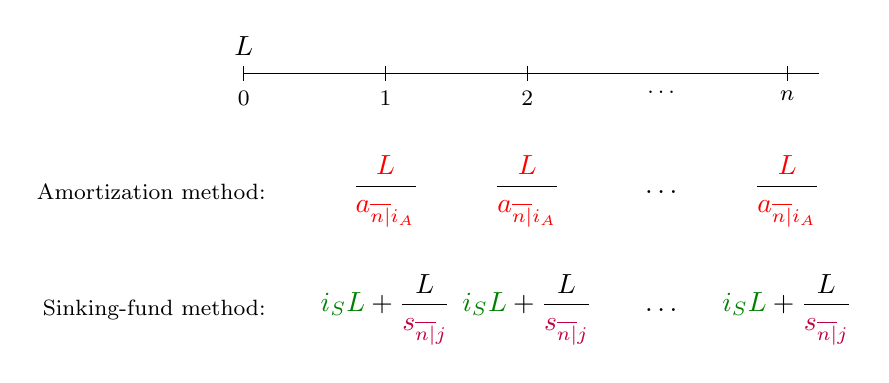
\begin{tikzpicture}
  \draw (0,0) -- (7.3,0);
  \foreach \x/\t in {0/0, 1.8/1, 3.6/2, 5.3/\ldots, 6.9/n} \node[below] at (\x,-0.1) {\footnotesize $\t$};
  \foreach \x in {0,1.8,3.6,6.9} \draw (\x,0.1) -- (\x,-0.1);
  \node[above] at (0,0.1) {$L$};
  \node[anchor=east] at (0.4,-1.5) {\footnotesize Amortization method:};
  \node[anchor=east] at (0.4,-3) {\footnotesize Sinking-fund method:};
  \foreach \x in {1.8,3.6,6.9} \node at (\x,-1.5) {$\dfrac{\red{L}}{\red{a_{\ang{n}i_A}}}$};
  \node at (5.3,-1.5) {$\ldots$};
  \foreach \x in {1.8,3.6,6.9} \node at (\x,-3) {$\green{i_S L} + \dfrac{L}{\purple{s_{\ang{n}j}}}$};
  \node at (5.3,-3) {$\ldots$};
\end{tikzpicture}
\end{center}

\end{frame}

\begin{frame}{Cash flow comparison, continued}

\textbf{When $i_A = i_S = j$:}
\begin{itemize}
\item Periodic payment under amortization method: $\red{\dfrac{L}{a_{\ang{n}j}}}$
\item Periodic payment under SF method:
\end{itemize}
\begin{align*}
\green{jL} + \purple{\frac{L}{s_{\ang{n}j}}} &= L\left(j + \frac{j}{(1+j)^n - 1}\right) = L\left(\frac{j(1+j)^n - j + j}{(1+j)^n - 1}\right) \\
&= L\left(\frac{j}{1 - v^n}\right) = \frac{L}{a_{\ang{n}j}}
\end{align*}

\begin{center}
\red{In this case, the two methods are equivalent}
\end{center}

\end{frame}

\begin{frame}{Cash flow comparison, continued}

\textbf{When $i_A = i_S$ and $i_S > j$:}
\begin{itemize}
\item Periodic payment under amortization method: $\red{\dfrac{L}{a_{\ang{n}i_S}}}$
\item Periodic payment under SF method:
\end{itemize}
\[
\green{i_S L} + \purple{\frac{L}{s_{\ang{n}j}}} > i_S L + \frac{L}{s_{\ang{n}i_S}} = \frac{L}{a_{\ang{n}i_S}}
\]

\vfill
\begin{center}
\red{Amortization method is better for the borrower.}
\end{center}
\vfill

\end{frame}

\begin{frame}{Cash flow comparison, continued}

\textbf{When $i_A = i_S$ and $i_S < j$:}
\begin{itemize}
\item Periodic payment under amortization method: $\red{\dfrac{L}{a_{\ang{n}i_S}}}$
\item Periodic payment under SF method:
\end{itemize}
\[
\green{i_S L} + \purple{\frac{L}{s_{\ang{n}j}}} < i_S L + \frac{L}{s_{\ang{n}i_S}} = \frac{L}{a_{\ang{n}i_S}}
\]

\vfill
\begin{center}
\red{Sinking fund method is better for the borrower.}
\end{center}
\vfill

\end{frame}

\begin{frame}{Other considerations}

A borrower may still choose the sinking fund method even if the periodic cost of payment is higher than under the amortization method because:
\begin{itemize}
\item The borrower controls the SF deposit amount. If it needs to reduce payments for a while, it can catch up later.
\medskip
\item The borrower can take risk in investing the deposits and maybe earn a higher return.
\medskip
\item The borrower can usually negotiate a lower loan rate than with amortization.
\end{itemize}

\end{frame}

\begin{frame}{Example 5.9}

A loan of 100,000 is to be repaid by 10 payments beginning one year after the loan is made.
\begin{itemize}
\item If the borrower chooses the amortization method, the lender charges a loan rate of 11\%.
\medskip
\item If the borrower chooses to pay interest only on the loan, the lender is willing to reduce the loan rate to 10\%. The borrower can get a savings rate of 8\%.
\end{itemize}

\medskip
Which one should the borrower choose?

\vfill
\end{frame}

\begin{frame}{Example 5.9, continued}

\vfill
\end{frame}

\begin{frame}{General equivalence}

\begin{itemize}
\item Suppose a loan is repaid using the sinking fund method, with loan rate \green{$i_S$} and savings rate \purple{$j$}.
\medskip
\item Let \red{$i'$} be the loan rate under the amortization method that makes the periodic cost of debt equal under the two methods:
\[
\green{i_S} L + \frac{L}{s_{\ang{n}\purple{j}}} = \frac{L}{a_{\ang{n}\red{i'}}}
\]
\item Approximate this loan rate as $\red{i' = i_S + \dfrac{i_S - j}{2}}$.
\end{itemize}

\end{frame}

\end{document}
